\documentclass{article}
\usepackage[letterpaper,hmargin={2.4cm,2.4cm},vmargin={2.4cm,2.4cm}]{geometry}
\usepackage[pdftex,hidelinks]{hyperref}
\usepackage{soul}
\usepackage{graphicx}
\usepackage{amsmath}

\usepackage{pdflscape}

\begin{document}
\title{Appendix A: Simulation Details and Results}
\date{} 
\maketitle
\renewcommand*\thetable{A\arabic{table}}
\renewcommand*\thefigure{A\arabic{figure}}
\renewcommand*\theequation{A\arabic{equation}}

\section*{Details}
\subsection*{Proof of Concept Simulation Study}

We used the \textbf{R} package \texttt{unmarked} to estimate the parameters 
for each simulation with the same
initial abundance (Poisson) and dynamics models as were simulated.
When run in a maximum likelihood framework, these models require a
a finite upper bound $N_{max}$; we used 200.  

\subsection*{Robustness Simulation Study}
For the geometric-recruitment simulation, we ran 1000 simulations with the following input 
parameters: $\Lambda = 10$, $\omega = \gamma = 0.5$, and $p = 0.25$.  
For the maximum likelihood exponential and geometric-recruitment models fit to these data, 
we used finite upper bound $N_{max} = 200$. 
For the Leslie matrix simulation, we also ran 1000 simulations with $\Lambda = 10$ and $p = 0.25$,
and we increased the number of sites to 200 and the number of years to 50.  We used
six age classes with apparent annual survival probabilities ($S_{i}$) of 0.32, 0.64, 0.68, 0.68, 0.64, and 0.56,
and fecundities ($m_{i}$) of 0.71, 1, 1.35, 1.7, 2.05, and 2.4.  This can be expressed as the post-breeding
census Leslie matrix model:
\begin{equation}
A = \begin{bmatrix} 0.2272 & 0.64 & 0.918 & 1.156 & 1.312 & 1.344 \\ 
0.32 & 0 & 0 & 0 & 0 & 0 \\
0 & 0.64 & 0 & 0 & 0 & 0 \\
0 & 0 & 0.68 & 0 & 0 & 0 \\
0 & 0 & 0 & 0.68 & 0 & 0 \\
0 & 0 & 0 & 0 & 0.64 & 0 \end{bmatrix}
\label{eq:leslie}
\end{equation}
We incorporated demographic stochasticity into this model with binomial distribution for survivals
(lower sub-diagonal of Eq.~\ref{eq:leslie}) and Poisson draws for fertilities (top row of 
Eq.~\ref{eq:leslie}).  Counts and initial abundances were based on adults (i.e. all age classes except
the first).  The starting age distribution was random Poisson with mean at the stable age distribution.
For the maximum likelihood exponential and geometric-recruitment models fit to these data, 
we used finite upper bound $N_{max} = 150$. 

The third simulation was a Gompertz model with two non-overlapping generations per year (sampling occasion).   
We used 200 sites for 25 years, and data-generating values of $\Lambda = 10$, $r = 0.05$, $K = 10$, and $p = 0.5$.
We estimated parameters with the Gompertz model with 
one generation per year using both maximum likelihood and MCMC approaches, as well
as allowing for two generations per year with MCMC.  
For the maximum likelihood model, we used finite upper bound $N_{max} = 150$. 
For the Bayesian framework we used non-informative priors ($\Lambda$ and $K  \sim \mathrm{U}(0, 30)$, $r  \sim \mathrm{U}(0, 5)$,
and $p  \sim \mathrm{U}(0, 1)$.  
For model and simulation we ran a single chain. We sampled the MCMC for 20,000 iterations, after 1,000 adaptation and tuning samples.  

We compared the bias, root mean
squared error, and coverage of all three model estimates.  For the models fit with MCMC,
bias and root mean squared error are based on the relationship between mean estimates
and true values, and coverage
based on percentage of 95\% credible intervals for parameters that overlap the true values.
\newpage

\begin{table}[t]
  \centering
\caption{Changed parameter values, by series of simulations.  We
simulated 1000 sets of data each combination of parameter values
for 100 sites over 40 years.  We assumed that initial abundance
($\Lambda$) was Poisson distributed.  For the exponential 
simulations we included all combinations of low, medium, and
high $\Lambda$, growth rate ($r$), and detection probability ($p$).
For the Ricker model simulations we used $\Lambda$ = 10 and $p$ = 0.25, and
simulated low, medium, and high values of $r$ and equilibrium density ($K$).
For the Ricker + immigration dynamics model we fixed all parameters the
same as the Ricker model (with $r$ = 0.05 and $K$ = 10) and
simulated low, medium, and high values of immigration rate ($\iota$).}  
\begin{tabular}{lcccccccc}
    \hline
    & \multicolumn{3}{c}{Exponential Growth} && \multicolumn{2}{c}{Ricker} &&
    Ricker + Immigration \\
    \cline{2-4}     \cline{6-7}    \cline{9-9}
& $\Lambda$ & $r$ & $p$ && $r$  & $K$ && $\iota$  \\    
\hline
    Low	        &1	&-0.01	&0.05	&&0.005	 &5	&&0.005  \\
    Med	        &5	&0	&0.25	&&0.05	&10	&&0.05   \\
    High		 &10 &0.005	&0.5	&&0.1	&20	&&0.5    \\
    \hline
  \end{tabular}
\end{table}


\begin{landscape}

\begin{table}[htb]
  \centering
  \footnotesize
  \caption{Simulation results from 27 cases of exponential dynamics with 1000 Monte Carlo replicates for each.}
  \begin{tabular}{cccccccccccc}
    \hline
    \multicolumn{3}{c}{Data generating values}&
    \multicolumn{3}{c}{Mean} &
    \multicolumn{3}{c}{RMSE} &
    \multicolumn{3}{c}{Coverage} \\
    \multicolumn{3}{c}{\rule{4cm}{1pt}} &
    \multicolumn{3}{c}{\rule{4cm}{1pt}} &
    \multicolumn{3}{c}{\rule{4cm}{1pt}} &
    \multicolumn{3}{c}{\rule{4cm}{1pt}} \\
    $\Lambda$ & $r$ & $p$ & $\Lambda$ & $r$ & $p$ & $\Lambda$ & $r$ &
    $p$ & $\Lambda$ & $r$ & $p$ \\
    \hline
10	&-0.005	&0.05	&10.03924	&-0.00601	&0.05007	&1.05051	&0.00605	&0.00432	&0.959	&0.945	&0.96\\
10	&-0.005	&0.25	&10.0333	&-0.00573	&0.25&0.76926	&0.00598	&0.01545 &0.951	&0.942	&0.945\\
10	&-0.005	&0.5	&10.00858	&-0.00598	&0.49984	&0.61057	&0.00532	&0.02352	&0.949	&0.957	&0.945\\
10	&0.005	&0.05	&10.06802	&0.00424	&0.04996	&1.04574	&0.00576	&0.00428	&0.955	&0.939	&0.949\\
10	&0.005	&0.25	&10.03648	&0.00399	&0.25087	&0.80109	&0.00525	&0.01665	&0.934	&0.954	&0.921\\
10	&0.005	&0.5	&9.96719	&0.00431	&0.50244	&0.61777	&0.00492	&0.02539	&0.934	&0.957	&0.92\\
10	&0	&0.05	&10.06548	&-9e-04	        &0.05001	&1.06134	&0.00553	&0.0046	&0.961	&0.96	&0.944\\
10	&0	&0.25	&10.03522	&-0.00093	&0.25012	&0.76321	&0.00555	&0.01585	&0.953	&0.943	&0.936\\
10	&0	&0.5	&10.0036	&-0.00067	&0.50052	&0.58102	&0.00544	&0.02274	&0.949	&0.945	&0.948\\
1	&-0.005	&0.05	&1.04714	&-0.01254	&0.05045	&0.24087	&0.02411	&0.00915	&0.949	&0.953	&0.97\\
1	&-0.005	&0.25	&1.01614	&-0.01173	&0.25038	&0.15418	&0.02267	&0.02749	&0.952	&0.949	&0.945\\
1	&-0.005	&0.5	&1.01056	&-0.01136	&0.50008	&0.13529	&0.02287	&0.03846	&0.957	&0.936	&0.95\\
1	&0.005	&0.05	&1.0281	        &-5e-05	        &0.05032	&0.23616	&0.02057	&0.00954	&0.939	&0.948	&0.947\\
1	&0.005	&0.25	&1.01389	&-0.00143	&0.2502	&0.1609	&0.02246	&0.0268	&0.957	&0.937	&0.946\\
1	&0.005	&0.5	&1.00554	&-0.00114	&0.50194	&0.13693	&0.02064	&0.03746	&0.947	&0.945	&0.95\\
1	&0	&0.05	&1.03641	&-0.00685	&0.05017	&0.23656	&0.02457	&0.00928	&0.958	&0.934	&0.961\\
1	&0	&0.25	&1.01556	&-0.00587	&0.24993	&0.16434	&0.02134	&0.02592	&0.944	&0.945	&0.953\\
1	&0	&0.5	&1.00539	&-0.00533	&0.49994	&0.13367	&0.01982	&0.03812	&0.951	&0.947	&0.952\\
5	&-0.005	&0.05	&5.07525	&-0.00638	&0.04978	&0.65646	&0.00881	&0.00496	&0.945	&0.959	&0.965\\
5	&-0.005	&0.25	&5.02641	&-0.00619	&0.25013	&0.4727	&0.00779	&0.01735	&0.943	&0.966	&0.937\\
5	&-0.005	&0.5	&5.01265	&-0.00656	&0.50067	&0.36154	&0.00814	&0.02465	&0.96	&0.949	&0.961\\
5	&0.005	&0.05	&5.05623	&0.00396	&0.05002	&0.62418	&0.00786	&0.00505	&0.944	&0.957	&0.952\\
5	&0.005	&0.25	&5.01567	&0.0041	&0.25014	&0.44585	&0.00746	&0.01723	&0.948	&0.947	&0.942\\
5	&0.005	&0.5	&5.02672	&0.00368	&0.49908	&0.36657	&0.00727	&0.02475	&0.947	&0.95	&0.943\\
5	&0	&0.05	&5.06304	&-0.00162	&0.04994	&0.61073	&0.00838	&0.00492	&0.96	&0.96	&0.956\\
5	&0	&0.25	&5.04372	&-0.00141	&0.24927	&0.46542	&0.00812	&0.01709	&0.942	&0.938	&0.945\\
5	&0	&0.5	&5.0239	&-0.00117	&0.4991	&0.37326	&0.00747	&0.02487	&0.952	&0.964	&0.946\\
  \hline
  \end{tabular}
  \label{tab:simexp}
\end{table}
\clearpage

\begin{table}
  \centering
  \footnotesize
  \caption{Simulation results from 9 cases of Ricker dynamics with 1000 Monte Carlo replicates for each.}
  \begin{tabular}{cccccccccccccccc}
    \hline
    \multicolumn{4}{c}{Data generating values}&
    \multicolumn{4}{c}{Mean} &
    \multicolumn{4}{c}{RMSE} &
    \multicolumn{4}{c}{Coverage} \\
    \multicolumn{4}{c}{\rule{4cm}{1pt}} &
    \multicolumn{4}{c}{\rule{4cm}{1pt}} &
    \multicolumn{4}{c}{\rule{4cm}{1pt}} &
    \multicolumn{4}{c}{\rule{4cm}{1pt}} \\
    $\Lambda$ & $r$ & $K$ & $p$ & $\Lambda$ & $r$ & $K$ & $p$ & $\Lambda$ & $r$ & $K$ &
    $p$ & $\Lambda$ & $r$ & $K$ & $p$ \\
    \hline
10	&0.005	&5	&0.25	&9.914 &0.00982  &6.368 &0.25211	&0.78540 &0.01147   &5.56126 &0.01614	&0.955 &0.807 &0.776 &0.963\\
10	&0.005	&10	&0.25	&9.954 &0.00866 &10.989 &0.25179 &0.77529 &0.00929   &8.73913 &0.01613  &0.960 &0.831 &0.828 &0.943\\
10	&0.005	&20	&0.25	&9.935 &0.00827 &59.778 &0.25145 &0.76079 &0.00830 &418.37837 &0.01559  &0.955 &0.841 &0.943 &0.955\\
10	&0.05	&5	&0.25	&10.038 &0.05290  &4.682 &0.25160 &0.89588 &0.02748   &1.58258 &0.01884  &0.945 &0.922 &0.919 &0.951\\
10	&0.05	&10	&0.25	&10.009 &0.05270  &9.718 &0.25172 &0.83411 &0.01876   &1.74552 &0.01742  &0.961 &0.930 &0.960 &0.948\\
10	&0.05	&20	&0.25	&10.000 &0.05136 &19.790 &0.25082 &0.83906 &0.01316   &2.51289 &0.01670  &0.951 &0.943 &0.962 &0.940\\
10	&0.1	&5	&0.25	&10.046 &0.10127  &4.833 &0.25048 &0.91333 &0.03529   &0.87551 &0.01953  &0.948 &0.954 &0.944 &0.954\\
10	&0.1	&10	&0.25	&9.990 &0.10254  &9.893 &0.25143 &0.88385 &0.02267   &0.89598 &0.01800  &0.949 &0.954 &0.964 &0.950\\
10	&0.1	&20	&0.25	&9.988 &0.10185 &19.916 &0.25117 &0.85780 &0.01543   &1.62111 &0.01680  &0.947 &0.941 &0.951 &0.953\\
  \hline
  \end{tabular}
  \label{tab:simricker}
\end{table}

\clearpage
\begin{table}
  \centering
  \footnotesize
  \caption{Simulation results from 3 cases of Ricker and immigration dynamics with 1000 Monte Carlo replicates for each.}
  \begin{tabular}{cccccccccccccccccccc}
    \hline
    \multicolumn{5}{c}{Data generating values}&
    \multicolumn{5}{c}{Mean} &
    \multicolumn{5}{c}{RMSE} &
    \multicolumn{5}{c}{Coverage} \\
    \multicolumn{5}{c}{\rule{4cm}{1pt}} &
    \multicolumn{5}{c}{\rule{7cm}{1pt}} &
    \multicolumn{5}{c}{\rule{7cm}{1pt}} &
    \multicolumn{5}{c}{\rule{4cm}{1pt}} \\
    $\Lambda$ & $r$ & $K$ & $\iota$ & $p$ & $\Lambda$ & $r$ & $K$ & $\iota$ & $p$ & $\Lambda$ & $r$ & $K$ &
    $\iota$ & $p$ & $\Lambda$ & $r$ & $K$ & $\iota$ & $p$ \\
    \hline
10 &0.05 &10 &0.005 &0.25  &9.997 &0.05148 &9.687 &0.00510 &0.25077 &0.87742 &0.01805 &1.77679 &0.00315 &0.01795  &0.951 &0.944 &0.964 &0.947 &0.942\\
10 &0.05 &10 &0.050 &0.25 &10.015 &0.05166 &9.758 &0.05039 &0.25070 &0.87490 &0.01731 &1.72376 &0.01055 &0.01839  &0.943 &0.932 &0.958 &0.940 &0.943\\
10 &0.05 &10 &0.500 &0.25 &10.000 &0.05057 &9.648 &0.50811 &0.25110 &0.96491 &0.01942 &2.68264 &0.07763 &0.02050  &0.947 &0.940 &0.952 &0.951 &0.941\\
  \hline
  \end{tabular}
  \label{tab:simricki}
\end{table}
\clearpage

\begin{table}[htb]
  \centering
  \footnotesize
  \caption{Parameters of geometric-recruitment simulation (1000 Monte Carlo replicates)
  and results of exponential and geometric-recruitment models fit to these data.}
  \begin{tabular}{lccccccccccccccccc}
    \hline
    & \multicolumn{5}{c}{Mean} &&
    \multicolumn{5}{c}{RMSE} &&
    \multicolumn{5}{c}{Coverage} \\
    \cline{2-6}     \cline{8-12}    \cline{14-18}
    Model & $\Lambda$ & $\gamma$ & $\omega$ & $r$\footnotemark[1] & $p$ &&
    $\Lambda$ & $\gamma$ & $\omega$ & $r$ & $p$ && 
    $\Lambda$ & $\gamma$ & $\omega$ & $r$ & $p$ \\
    \hline
Simulation & 
10	&0.5	&0.5	&0	&0.25	&&-	&-	&-	&-	&-	&&-	&-	&-	&-	&-\\
Exponential &
12.710	&-	&- 	&-0.00052 	&0.19728	&&
2.8808	&-	&- 	&0.00458	&0.05424	&&
0.130	&-	&- 	&0.957 	&0.039 \\
Geometric-recruitment &
10.457	&0.57321	&0.42621	&- 	&0.24269	&&
1.39877 &0.17905	&0.17944	&- 	&0.02925	&&
0.851	&0.935	&0.932	&- 	&0.814 \\
  \hline
  \multicolumn{18}{c}{$^{1}$ Derived parameter: $r = \log(\gamma + \omega)$.}
  \end{tabular}
  \label{tab:simgeom}
\end{table}

\clearpage

\begin{table}[htb]
  \centering
  \footnotesize
  \caption{Results of exponential and geometric-recruitment models fit to Leslie matrix simulation (1000 Monte Carlo replicates).}
  \begin{tabular}{lccccccccccccc}
    \hline
    & \multicolumn{5}{c}{Mean} &&
    \multicolumn{3}{c}{RMSE} &&
    \multicolumn{3}{c}{Coverage} \\
    \cline{2-6}     \cline{8-10}    \cline{12-14}
    Model & $\Lambda$ & $\gamma$ & $\omega$ & $r$\footnotemark[1] & $p$ &&
    $\Lambda$ & $r$ & $p$ && 
    $\Lambda$ & $r$ & $p$ \\
    \hline
Exponential &
27.841	&-	&- 	&-0.00470	&0.09037	&&
17.97942	&0.00186 	&0.15979	&&
0.000 		&0.977 	&0.000 \\
Geometric-recruitment &
12.782	&0.21211	&0.78326	&-	&0.19720	&&
2.92896 	&- 	&0.05438	&&
0.057		&- 	&0.022 \\
  \hline
  \multicolumn{14}{c}{$^{1}$ Derived parameter: $r = \log(\gamma + \omega)$.}
  \end{tabular}
  \label{tab:simmat}
\end{table}
\clearpage

\begin{table}[htb]
  \centering
  \footnotesize
  \caption{Parameters of Gompertz simulation with two generation per year 
(1000 Monte Carlo replicates)
  and results of models fit to these data.}
  \begin{tabular}{lcccccccccccccc}
    \hline
    & \multicolumn{4}{c}{Mean} &&
    \multicolumn{4}{c}{RMSE} &&
    \multicolumn{4}{c}{Coverage} \\
    \cline{2-5}     \cline{7-10}    \cline{12-15}
    Model & $\Lambda$ & $r$ & $K$ & $p$ &&
    $\Lambda$ & $r$ & $K$ & $p$ && 
    $\Lambda$ & $r$ & $K$ & $p$ \\
    \hline
Simulation & 
10	&0.05	&10	&0.5	&&-	&-	&-	&-	&&-	&-	&-	&-\\
Gompertz (MLE; 1 generation/year) &
8.392	&0.00919	&1.269	&0.60241	&&
1.64842	&-	&8.94192	&0.10395	&&
0.013	&-	&1.000 	&0.000 \\
Gompertz (MCMC; 1 generation/year) &
8.315	&0.03044	&4.575	&0.60723	&&
1.72224	&-	&5.70813	&0.10870	&&
0.007	&-	&0.368		&0.000 \\
Gompertz (MCMC; 2 generations/year) &
9.969	&0.05405	&10.407	&0.50337	&&
0.55084	&0.01697	&2.26087	&0.02318	&&
0.921	&0.964	&0.967	&0.935 \\
  \hline
  \end{tabular}
  \label{tab:simgomp}
\end{table}

\clearpage


\begin{figure}
\caption{Histograms of 1000 parameter estimates for each of nine
simulation cases with Ricker dynamics. The blue vertical lines are the 
data-generating values.}
  \centering
  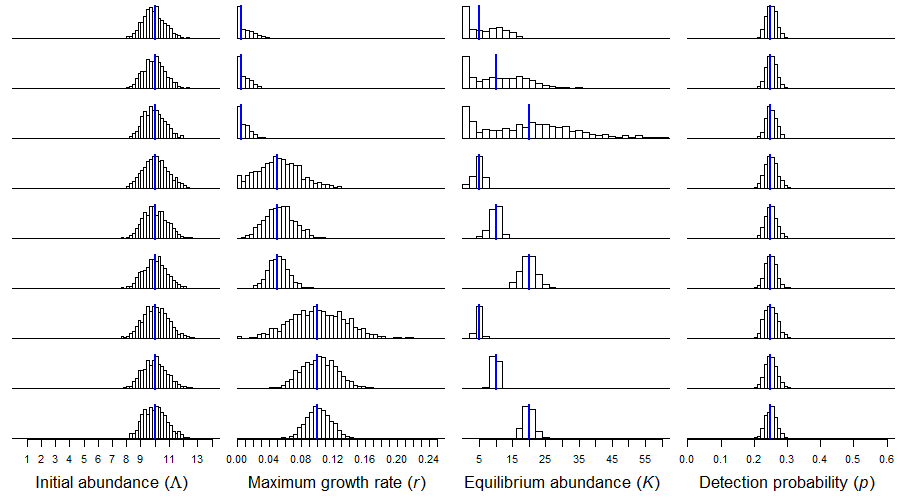
\includegraphics{../figs/rick_hists}
\label{fig:rick_hists}
\end{figure}

\begin{figure}
\caption{Histograms of 1000 parameter estimates for each of three
simulation cases with Ricker + immigration dynamics. The blue vertical lines are the 
data-generating values.}
  \centering
  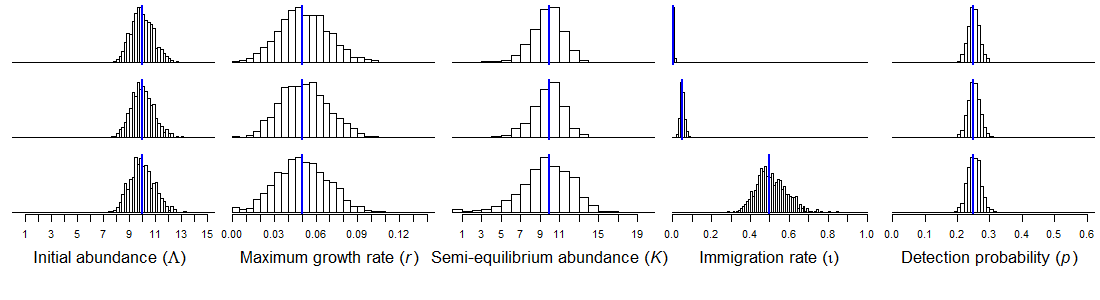
\includegraphics[width=8.5in]{../figs/ricki_hists}
\label{fig:ricki_hists}
\end{figure}

\begin{figure}
\caption{Histograms of 1000 parameter estimates for each of two
simulation cases with geometric-recruitment or Leslie matrix dynamics, each fit with 
exponential and geometric-recruitment models. The blue vertical lines are the 
data-generating values; the data-generating values for $r$ are derived from
the actual dynamic parameters of these models.  No data-generating values
are provided for $\gamma$ or $\omega$ by the Leslie matrix model because
each age class had its own survival and fecundity parameters.}
  \centering
  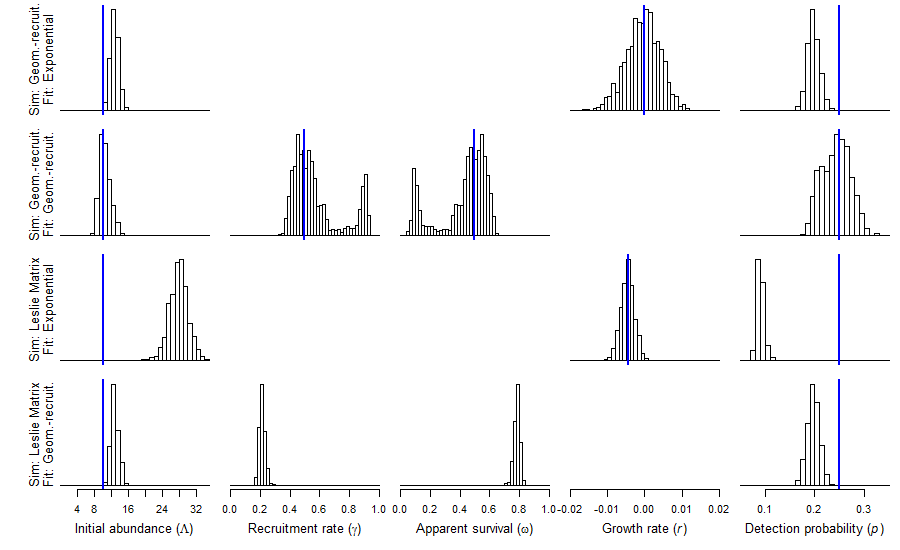
\includegraphics{../figs/geom_mat_hists}
\label{fig:geom_mat_hists}
\end{figure}

\begin{figure}
\caption{Histograms of 1000 parameter estimates simulated with Gompertz dynamics, 
two generations per year, fit with three different Gompertz models.
The vertical lines are the data-generating values; changing the number of generations
changes the meaning of $r$, so no data-generating values of it are provided for the 
single generation per year cases.}
  \centering
  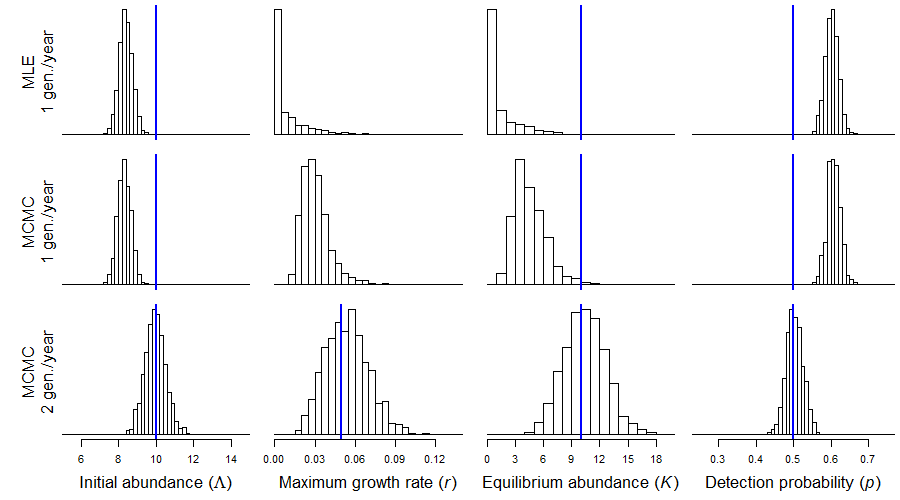
\includegraphics{../figs/gomp_hists}
\label{fig:gomp_hists}
\end{figure}
\end{landscape}

\end{document}
